\documentclass[11pt]{article}
\usepackage{icmlko}
\begin{document}

\title{깊이가 원핫을 산다 --- 그리고 죽었던 손잡이가 자료가 자라자 되살아났다}
\author{월드모델 실험실}
\date{노트 405 · 2026년 8월 1일}
\maketitle

\begin{abstract}
노트 404가 도메인 원핫이 \textbf{정보를 하나도 안 더한다}는 것을 보였다 ---
관측 표시자 무늬만으로 열한 도메인 중 아홉이 순도 1.000 으로 갈린다.
그러면 남는 후보는 \textbf{편의}뿐이다: 원핫이 있으면 갈림 하나로 되는 일을,
없으면 표시자 서른네 열의 논리곱으로 다시 지어야 한다. 사전 등록했다 ---
\emph{편의가 맞으면 깊이가 원핫을 대신할 수 있어야 한다.}

\begin{center}
\begin{tabular}{lrrrr}
\hline
 & 원핫O 깊이4 & 원핫X 깊이4 & 구멍 & \textbf{원핫X 최고} \\
\hline
아이돌 & $+0.1981$ & $+0.0292$ & $0.1689$ & $\mathbf{+0.2424}$ (깊이 8) \\
게임 & $+0.6085$ & $+0.5524$ & $0.0561$ & $\mathbf{+0.6248}$ (깊이 12) \\
\hline
\end{tabular}
\end{center}

\textbf{구멍이 메워지는 정도가 아니라 넘친다} --- 아이돌 \textbf{126\%},
게임 \textbf{129\%}. 원핫 없이 깊이만 준 모형이 원핫 있는 깊이 4 모형을
\textbf{이긴다.} 판이 깊이로 움직인 폭도 원핫 없는 쪽이 크다($0.0224$ 대
$0.0167$) --- 예측한 상호작용이다. \textbf{노트 401이 열어 둔 물음이
닫힌다: 원핫이 파는 것은 정보가 아니라 편의다.}

그리고 예상 못 한 것이 딸려 나왔다. \textbf{깊이 $4 \to 6$ 이 원핫이 있어도
판을 $+0.0167$ 올린다}($0.4430 \to 0.4597$). \textbf{노트 272가 깊이를
죽였던 손잡이다.}
\end{abstract}

\section{죽은 손잡이가 왜 살아나나}

노트 216이 알파를, 216·243이 $\tau$ 를, \textbf{272가 깊이를} 죽였다.
노트 396이 $K$ 를 살리면서 적은 이유는 ``$K$ 는 봉우리가 없는 순수 비용
손잡이''였다 --- 깊이는 봉우리가 있어 안쪽에서 고르면 빗나간다.

그 뒤로 자료가 자랐다. 이번 사이클에만 만화 $+4{,}999$ · 웹툰 $+835$ ·
애니 $+1{,}382$ 행이 들어왔고 펀딩 표본이 교정됐다. \textbf{봉우리의
자리는 자료 크기의 함수다} --- 행이 적을 때 깊이 6 이 과적합이던 것이,
행이 늘면 과적합이 아니게 된다. 가설: \textbf{손잡이는 자료가 자라면
되살아난다. 한 번 죽은 손잡이를 영영 죽은 것으로 두면 안 된다.}

깊이 $6 \cdot 8 \cdot 12$ 는 평평하다($0.4597 / 0.4586 / 0.4596$) ---
\textbf{무릎이 6} 이고, 그 위는 다시 봉우리 없는 평지다.

\section{아직 안 정해진 것}

위 수치는 전부 \textbf{$K{=}8$} 에서 씨앗 넷을 평균한 것이다. 챔피언은
$K{=}32$ 다. \textbf{사전 등록하고 관문을 돌리는 중이다} --- 깊이 6 이
깊이 4 를 $+0.003$ 이상 · 부호 $\ge 9/12$ 로 이기면 채택.

\textbf{미리 적은 실패 조건}: \emph{$K{=}8$ 에서만 나는 이득일 수 있다.}
자루가 여덟뿐이면 분산이 커서 깊은 나무가 그것을 대신 메운다. $K{=}32$ 는
이미 배깅으로 분산을 줄여 놨으니 깊이가 살 자리가 없을 수 있다. 그러면
이것은 깊이의 부활이 아니라 \textbf{자루의 대체물}이고 노트 272는 그대로
산다.

\section{남은 것}

\begin{tabular}{lp{7.2cm}}
\hline
죽은 손잡이 다시 쓸기 & 깊이가 살아났다면 알파와 $\tau$ 도 다시 봐야 한다.
자료가 자란 뒤로 아무도 안 재 봤다 \\
원핫을 아예 뗄까 & 깊이 8 이면 원핫 없이도 아이돌이 더 낫다. 노트 399의
맞바꿈(판 $0.0117$ 내고 전이 $+0.2058$)이 \textbf{깊이로 공짜가 될} 수 있다
--- 이번 사이클에서 처음으로 벽이 아닐 수 있는 길 \\
\hline
\end{tabular}

\begin{figure}[h]
\centering
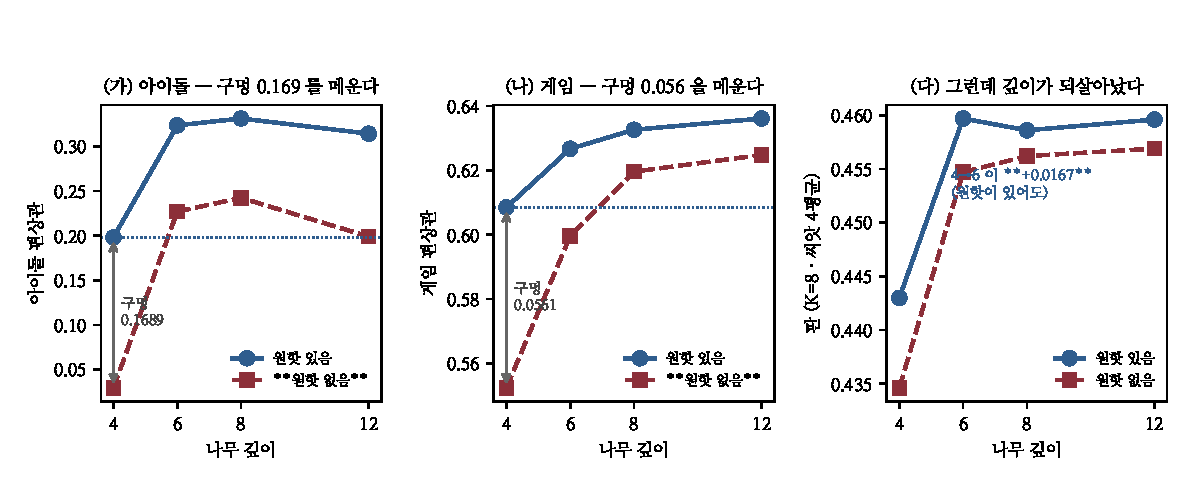
\includegraphics[width=\textwidth]{figs/fig405.pdf}
\caption{(가)(나) 원핫 없는 팔(붉은 파선)이 깊이를 올리면 원핫 있는 깊이 4
수준(파란 점선)을 넘어선다. (다) 깊이 $4 \to 6$ 은 원핫이 있어도 판을
올린다 --- 노트 272가 죽인 손잡이다. 전부 $K{=}8$ · 씨앗 4평균.}
\end{figure}

\end{document}
